\section{Some Basic Op-Amp Circuits}
\label{lab_op-amps}

%\makelabheader %(Space for student name, etc., defined in master.tex)

\bigskip

\begin{enumerate}[wide]

\item The circuit below on the left shows a non-inverting amplifier with a gain of 2.  If $V_{in} = 2$~volts, what are $V_+$, $V_-$, and $V_{out}$?  Modify this circuit to have a gain of 5, and test it out. (Note: The diagram on the right shows the ``pin-out'' for the LM324 op-amp chip; other pin-out diagrams are in Appendix \ref{appendix_pinouts}.  Place the LM324 on your breadboard straddling the center line so that you have four additional holes connected to each pin.)
%\vspace{-0.1in}
\begin{center}
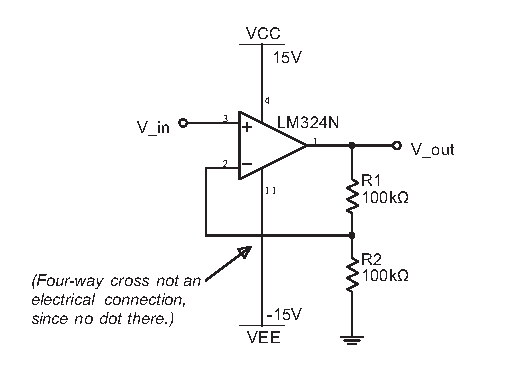
\includegraphics{op-amps/noninverting.eps}
\hspace{0.2in}
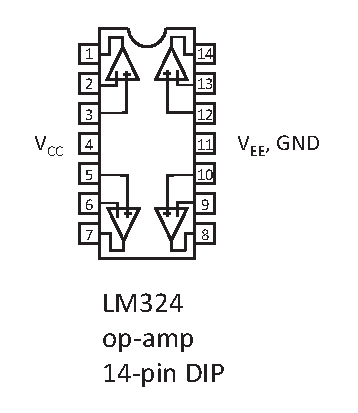
\includegraphics[scale=0.8]{appendices/pinouts/lm324.eps}
\end{center}


\item The circuit below is an inverting amplifier with a gain of $-1$.  (The power supplies $V_{CC}$ and $V_{EE}$ have been omitted from the diagram for clarity, as they often are, but they still have to be connected or it won't work.)  If $V_{in}$ is 2 volts, what is $V_-$ (at the negative terminal), and what should be the current through $R_4$?  Modify the circuit to have a gain of $-5$, and test it out.  
\begin{center}

\includegraphics{op-amps/inverting.eps}
\end{center}

\item Set your function generator to output a 1~kHz sine wave with an (open circuit) RMS voltage of about 100~mV.  (Measure it with your oscilloscope.)  What happens to that RMS voltage when you connect the function generator to your speaker?  The new RMS voltage will be quite small.  To measure it accurately, you will need to have your probe on 1x, trigger off of your TTL signal, and also use the ``Average'' function on your oscilloscope, under the ``Acquire'' menu.  What is this ``averaging,'' and how does it help you?  Set it back to ``Sample'' when you're done, or you'll get weird results later.

\item From your measurement above and the known output impedance of your function generator, calculate the input impedance of the speaker.  (This is similar to what you did in Lab~\ref{lab_input_output_impedance}, part~\ref{part_func_gen_impedance}.)  What is the average power being dissipated in the speaker?  Is it audible? \label{part_nobuffer}

\item The circuit below is called a ``buffer.'' What is its output, and why the heck would you ever want to build such a thing?  Insert this buffer into your circuit for part~\ref{part_nobuffer}, with the output of the function generator as $V_{in}$, and the $V_{out}$ connected to the speaker.  Now what is the RMS voltage across the speaker?  And the average power dissipated in the speaker?  What are the apparent input and output impedances of this amplifier?  On a scale of 1 to 10, how cool is this? \label{part_buffer}
\begin{center}

\includegraphics{op-amps/buffer.eps}
\end{center}


\item While monitoring both the $V_{in}$ and $V_{out}$ on your oscilloscope for the circuit in part~\ref{part_buffer}, gradually increase the amplitude of the signal generator.  How do $V_{in}$ and $V_{out}$ change?  What is the maximum current through the speaker?  Is this consistent with the value listed on the data sheet of the LM324? 

\begin{minipage}{.50\textwidth}
\item The circuit to the right is a variation on the inverting amplifier called a summing amplifier, where the output is given by 
\begin{equation*}
V_{out} = -R_F \left( \frac{V_1}{R_1} + \frac{V_2}{R_2} +\frac{V_3}{R_3} \dots \right).
\end{equation*}
One place where such a circuit is useful is as a digital to analog (``D-to-A'') converter.  Suppose 
\end{minipage}
\begin{minipage}{.49\textwidth}
\begin{flushright}
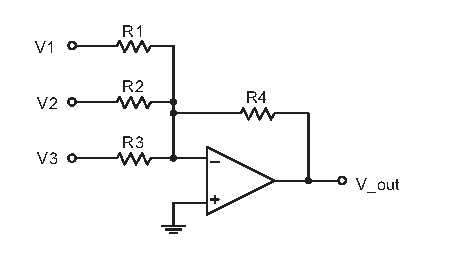
\includegraphics{op-amps/summing_amp.eps}
\vspace*{0.2in}
\end{flushright}
\end{minipage}
you have four digital inputs, whose voltages are all either +5 volts (for a logical ``1'') or 0 volts (for a logical ``0'').  These inputs represent the ``ones place,'' the ``twos place,'' the ``fours place,'' and the ``eights place'' of a single number expressed in base two, so that ``0001'' is 1, ``0010'' is 2, ``0011'' is 3, and so on.  Show how to use a summing amplifier as part of a 4-bit D/A converter, where the analog output ranges from 0 to +15 volts, corresponding to the numbers 0 through 15.  Note that the output of your summing amplifier will be a negative voltage; how can you make it positive?  (Also: you'll use this circuit again in part~\ref{part_proportional_controller} of this lab, so don't destroy it when you're done.) \label{part_summer}
%\begin{center}
%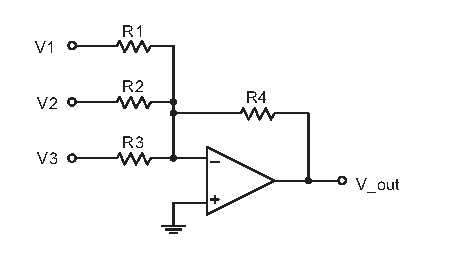
\includegraphics{op-amps/summing_amp.eps}
%\end{center}

\begin{minipage}{.53\textwidth}
\item The circuit to the right shows an example of a differential amplifier; for the case where both $R_1$'s and $R_2$'s are the same, the output is given by  \label{part_differential}
\begin{equation*}
V_{out} = \frac{R_2}{R_1} \left( V_2 - V_1 \right).
\end{equation*}
Use a differential amplifier like the one shown to create a triangle wave that sweeps between $-8$ and
\end{minipage}
\begin{minipage}{.46\textwidth}
\begin{flushright}
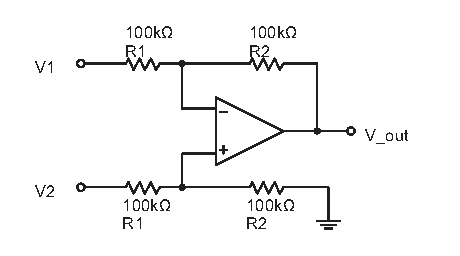
\includegraphics{op-amps/differential_amp.eps}

\vspace*{0.32in}
\end{flushright}
\end{minipage}
0 volts.  You can use the output of your function generator (set to whatever amplitude you want) and the output from your 5V DC supply, and you can change the values of the resistors $R_1$ and $R_2$ to whatever you like.  
%\begin{center}
%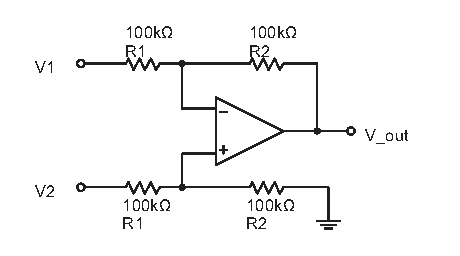
\includegraphics{op-amps/differential_amp.eps}
%\end{center}

\pagebreak[4]
\item (This part is intended to be long and complicated!)  Your job is to design, build and test a ``proportional controller,'' which could in principle be used to maintain a hotplate at a constant temperature.
\begin{itemize}[nosep]
\item The temperature desired by the user (the ``setpoint temperature'') will be represented by an adjustable voltage which varies between 0 and 1.5 volts, set by a D-to-A converter like you already made in part~\ref{part_summer} of this lab.  (You can imagine that in a more sophisticated implementation, those four bits might actually be set by some kind of digital keypad or something.)
\item The actual temperature will be read by a bridge circuit such as you built in Lab~\ref{lab_bridge}.  The difference $\Delta V_{AB}$ from the bridge should be amplified to a level that also ranges between roughly 0 and 1.5 volts as you warm one of the resistors with your fingers.
\item The output of your circuit should be proportional to the difference between those two voltages representing the setpoint temperature and the actual temperature.  (A proportionality constant of 1 is fine.)  Though you won't do it here, this output could be sent to a heater to maintain a constant, desired temperture.  Incidentally, the cruise control in a car works the same way, pressing the gas pedal down by an amount that is proportional to the difference between the desired speed and the actual speed.
\end{itemize}
Hint: you'll be in trouble if you hook up $V_A$ from the bridge circuit directly to the differential amplifier you made in part \ref{part_differential} because the amplifier's input impedance is too low.  How can you correct this? \label{part_proportional_controller}


\end{enumerate}

\textbf{Possible Exam Questions:}

\begin{itemize}

\item This is the first lab where you have been introduced to a truly new component (an op-amp) and several new kinds of circuits you can build with them.  In this lab, you were shown examples of each circuit and asked to measure or modify them.  On an exam, you won't have your hand held so much.  You are responsible for knowing every circuit that you have built here.

\begin{itemize}
\item If you are asked, ``Draw a non-inverting amplifier with a gain of 10,'' you will need to draw one from memory, choosing appropriate values for any resistors you use.

\item If you are asked, ``Design an 8-bit D-to-A converter,'' you will need to come up with a design similar to what you did in part~\ref{part_summer} of this lab.

\item Alternatively, you may be shown any of the circuit diagrams from this lab, and asked ``What does this do?'' or ``What is its input impedance?'' or ``What is the current through resistor $R_2$.''
\end{itemize}

\item Which has a greater input impedance: an inverting amplifier or a non-inverting amplifier?

\item Estimate the output impedance of a non-inverting amplifier.

\item When you build a non-inverting amplifier, you generally want to use resistors in the neighborhood of 10~k$\Omega$ to 100~k$\Omega$.  What could go wrong if you use values that are way too high, like 100~M$\Omega$?  What could go wrong if you use values that are way too low, like 10~$\Omega$?

\item From memory, what might be typical approximate values of an op-amp's (a) input and output impedances, (b) intrinsic gain, (c) maximum output current, and (d) slew rate?  

\item Describe how to measure small signals with an oscilloscope, including triggering, averaging, and probe settings.


\end{itemize}






